\documentclass{ltjsbook}
\usepackage{docmute} 
\usepackage{../../myStyle} 

\begin{document}
\chapter{Difference in Means between Two Groups}
\label{m20_ttest}

The most commonly used test in practical psychology is the test of mean differences. As we learned in experimental design, it is used in combination with RCT to consider the difference in group averages observed as the magnitude of the effect.
In this lecture, we will first consider testing the difference in means between two groups. In the case of two groups with related samples, it actually becomes a judgment about one "distribution of differences," so we can have the same discussion as before.
If there are two unrelated groups, the simplest case is the linear model. By connecting the discussion of factorial design (linear model) and statistical testing, it is possible to expand to multiple factorial designs.

\section{One Factor Within Design, 2 Levels}
Until now, we have explained the concept of the null hypothesis testing and its formalized procedure, as well as discussing specific ways of reporting and interpreting results through examples of testing for mean values and correlation coefficients.

This time, we will discuss testing the difference in means between two groups, which is one of the most commonly seen techniques in psychological research.
The basic framework of the experiment is to "observe the difference between the group that intervened and the group that did not intervene using the difference in the group means." It is a model to examine whether the "difference" in the mean values of two groups, the experimental group and the control group, was significant or not.

In terms of experimental design, this can be referred to as a single-factor, between-subjects, 2-level design. If you are unsure about the terms factor, between/within groups, and level, please refer back to the material covered in chapter \ref{m12_design1}.

In this section, we will first discuss the experimental design of a single factor or within-group design, specifically for a two-level plan. This design involves within-group or repeated measures, and with only two levels, it is an experimental design to determine if there was an effect or not before and after intervention. To be more precise, within-group design includes not only repeated measures but also cases where there is a correspondence with the data. In the case of investigating twins or two individuals in a close relationship (which is generally referred to as an intimate relationship in social psychology, and is a good term that is not limited to gender), there may be a correlation between the two variables since there is a correspondence between the pairs and they may be mutually influenced. In such situations, it is necessary to analyze while also considering the underlying factors that they share. Within-group design is also sometimes referred to as "paired analysis".

Let's say this is a study that collects pre- and post-data. For example, if we are looking at psychological well-being, we would conduct a survey beforehand, then administer some sort of clinical intervention (such as training in relaxation techniques), followed by another survey of the same individuals after a certain period of time (see Figure 19.01).

\begin{figure}[ht]
   \centering
   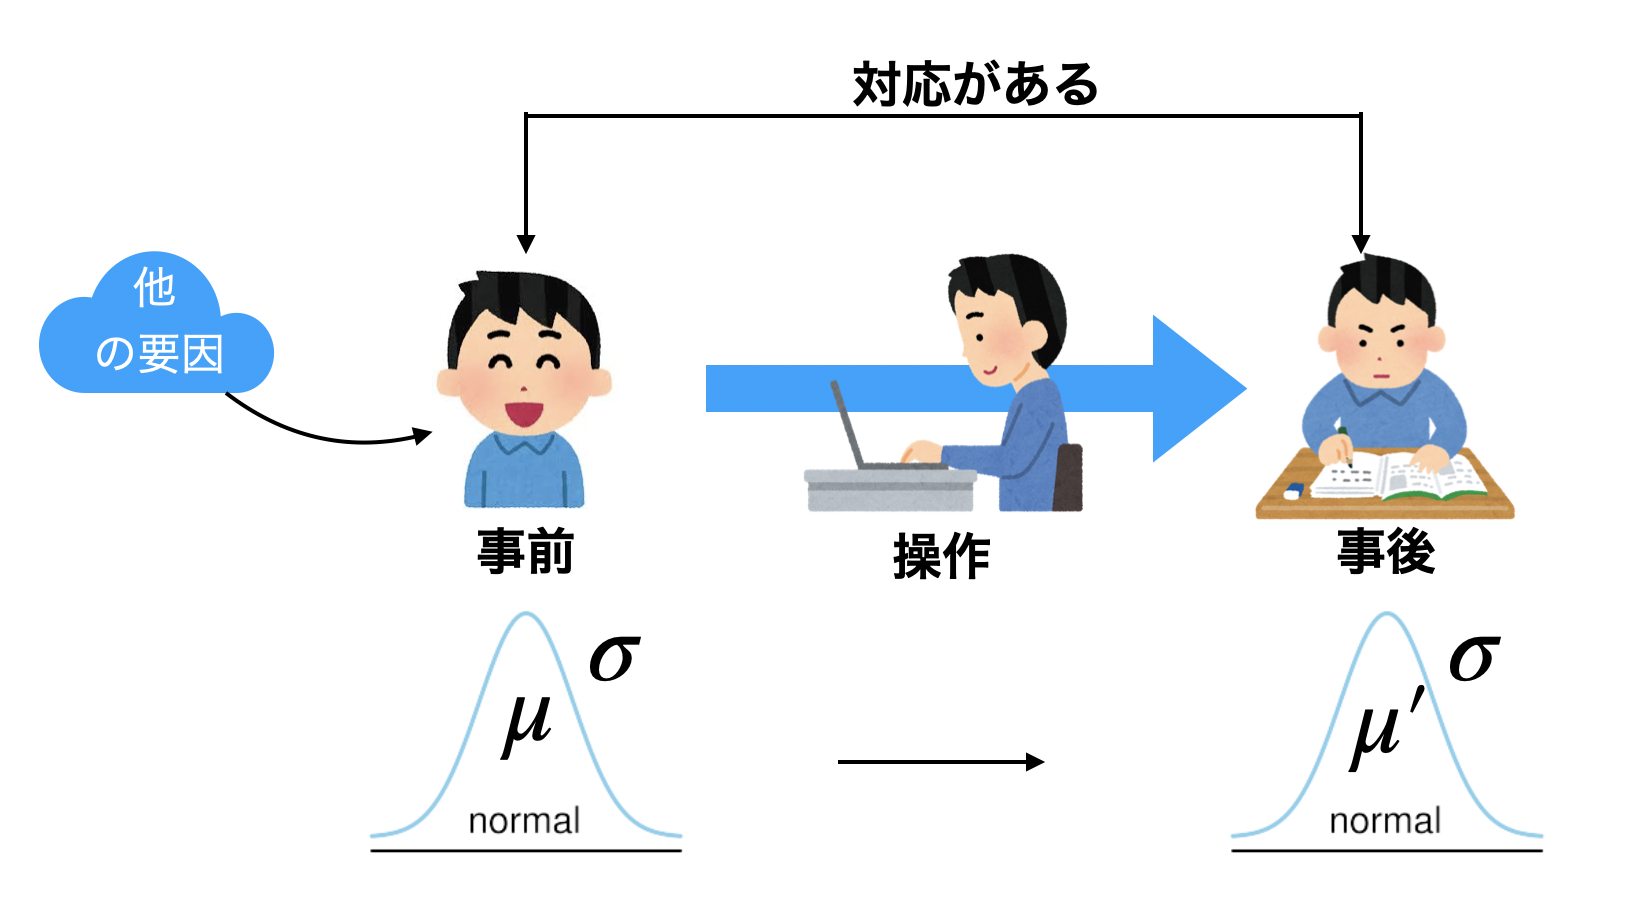
\includegraphics[keepaspectratio,width=0.8\linewidth]{../images/19_NHST2/slide19_01.png}
   \caption{一要因群内2水準の実験モデル}
   \label{fig::19_01}
\end{figure}


Assuming that the subjects were collected randomly from the population, and the pre-survey health status scores followed a normal distribution. If we conducted the same test afterwards and observed an overall effect despite individual differences, we could conclude that the clinical intervention method is excellent. While individual client changes are important, it is natural to want to verify changes in the population and the difference in population means by borrowing the power of inferential statistics, to interpret the effect more generally. Therefore, we estimate the population mean from the sample mean and assume that the population distribution is normal, and we can also assume the range of sample mean variations by using this. Using this, we want to estimate the possible location of the population mean and consider how it differs between pre- and post-interventions. Here, since we do not know the population mean or standard deviation, we consider the unbiased variance calculated from the sample to be an estimated value. In estimation from the sample statistic, it follows not a normal distribution but a t-distribution, so we also estimate this using a t-distribution. We consider using this estimate for testing, and in particular, this test is called the t-test.


I would like to know if there have been any changes before and after, and fortunately, it is known that the difference of the probability variables $X$ and $Y$ that follow the normal distribution, $X-Y$, also follows the normal distribution. Since there is correspondence in the data this time, I can use this feature to determine whether there have been any changes before and after.

As a numerical example, let's consider the following two groups (Table \ref{tbl19::01}).
% latex table generated in R 4.0.2 by xtable 1.8-4 package
% Wed Sep  2 09:32:58 2020
\begin{table}[ht]
	\centering
	\caption{Pre-Post Design Data}
	\begin{tabular}{rrrrrrrrrrr}
		\hline
		Participants & 1  & 2  & 3  & 4  & 5  & 6  & 7  & 8  & 9  & 10 \\
		\hline
		pre          & 34 & 25 & 13 & 21 & 13 & 26 & 19 & 12 & 19 & 19 \\
		post         & 35 & 30 & 16 & 27 & 20 & 28 & 16 & 14 & 18 & 21 \\ \hline
		diff         & 1  & 5  & 3  & 6  & 7  & 2  & -3 & 2  & -1 & 2  \\
		\hline
	\end{tabular}
	\label{tbl19::01}
\end{table}

You are a translator. 

There are 10 experiment participants here. Table \ref{tbl19::01} shows their pre- and post-scores and the differences. To express this in formula form, let the pre-score be $X_1$ and the post-score be $X_2$. Then the difference $D$ is given by
\[ D = X_2 - X_1 \]
However, regarding its average as well...
\[ \bar{D} = \bar{X_2} - \bar{X_1} \]
This implies that the variable $D$ follows a normal distribution with mean $\mu_D$ and standard deviation $\sigma_D$. Furthermore, the TeX code will not be modified.
\[ D \sim N(\mu_D,\sigma_D)\]
From
\[ \bar{D} \sim N(\mu_D,\frac{\sigma_D}{\sqrt{n}}) \]
You are a translator. 

The text in Japanese says: "Assuming that we know $\sigma_D$, we can simply use its unbiased estimator, which is the sample variance of $D$, denoted by $s_D^2$."
\[ t = \frac{\bar{D}-\mu_D}{\hat{\sigma_D}/\sqrt{n}} \]
This means that it follows a t-distribution with degrees of freedom of $n-1$. If there are people who don't quite understand this series of steps when expressed in mathematical equations, please refer back to Chapter \ref{m17_estimation_and_test} for confirmation.

Let's do interval estimation before the hypothesis test. The 95\% interval of the $t$-distribution with $n-1=10-1=9$ degrees of freedom is $\pm 2.262157$\footnote{Just to make sure, in R, we would use \texttt{qt(0.975,df=9)}.} . Therefore, using this value, we can conclude that
\[ -2.262 < \frac{\bar{D}-\mu_D}{\hat{\sigma_D}/\sqrt{n}} < 2.262 \]
Without modifying the TeX code, please translate the following Japanese text into English:

Next, multiply both sides by the denominator.
\[ -2.262 \times \hat{\sigma_D}/\sqrt{n} < \bar{D}-\mu_D < 2.262 \times \hat{\sigma_D}/\sqrt{n} \]
Move $\bar{D}$ to the other side of the equation.
\[ \bar{D}-2.262 \times \hat{\sigma_D}/\sqrt{n} < \mu_D < \bar{D}+2.262\times \hat{\sigma_D}/\sqrt{n} \]
As $\bar{D} = 2.400$ and $\hat{\sigma_D} = 3.062$ here,
\[ 0.2097 < \mu_D < 4.590 \]
It can be seen that although the difference in sample means was 2.4 points, the estimated difference in population means was 2.4 points with a 95% confidence interval of [0.21, 4.59]. In other words, even with a conservative estimation within the 95% interval, there is a difference of at least 0.21 points, indicating that there is indeed a difference.

Let's put this on the logic of testing.
\paragraph{Setting the Hypothesis} Both null hypothesis and alternative hypothesis are needed. The null hypothesis is a hypothesis that there is no difference before and after, and no effect. In symbols, it is $\mu_D=0$. The alternative hypothesis is that there is a clinical effect, and the difference in the dependent variable should be zero plus. That is, $\mu_D > 0$.
\paragraph{Selecting the Test Statistic} Since we are estimating the mean value, the test statistic to be used is $t$.
\paragraph{Setting the Probability as the Criteria for Judgment} Let's set the significance level at $\alpha$ = 5\% for this decision.
\paragraph{Calculate the observed value of the test statistic}We did not previously calculate $\frac{\bar{D}-\mu_D}{\hat{\sigma_D}/\sqrt{n}} $ as we were performing an interval estimation. Let us do so now. \underline{Assuming the null hypothesis, $\mu_D=0$},
\[t= \frac{\bar{D}-\mu_D}{\hat{\sigma_D}/\sqrt{n}}  = \frac{2.4-0}{3.062/\sqrt{10}}  = 2.479\]
This $t=2.479$ follows the $t$-distribution with $9$ degrees of freedom. The probability of obtaining a $t$-value greater than or equal to this observed value is $p=0.0175$.
"Judge whether the initial hypothesis is incorrect or correct."
Since the value of t calculated under the null hypothesis is lower than the critical value of 5%, this indicates that it is a rare occurrence. Given this unusual result, it is possible that there is an error in the assumption that there is no significant difference. Therefore, we reject the null hypothesis and accept the alternative hypothesis.

The way of reporting the results is,
\begin{quote}
After conducting a corresponding t-test, it was statistically significant with $t(9)=2.479, p=0.0175$. 
\end{quote}

You are a translator.

By the way, do you remember the results of the confidence interval estimation we did earlier? Considering a 95\% margin, there might have been a difference of at least 0.21 or as much as 4.59. Since the lower end of the interval, which represents the minimum possible difference, is not zero (i.e., the null hypothesis), simply looking at this interval is enough to reject the null hypothesis. However, if the confidence interval spans zero, meaning that the minimum possible difference is negative (i.e., the opposite of what was expected) and the maximum possible difference is positive, a significance test would not be conclusive. This information from the confidence interval estimation also indicates the extent to which the estimated mean value could vary, and reporting this range along with the estimated mean can serve as a useful guide to the reliability of the experiment. Therefore, let's revise the previous report example as follows:

\begin{quote}
   After conducting a $t$-test with degrees of freedom $9$, the results show that $t(9)=2.479$, $p=0.0175$, and the $95\%$ confidence interval is $[0.21,4.59]$, indicating statistical significance.
\end{quote}


It would be even better\footnote{You may think that cutting at the 5% level or reporting the width of the 95% level is redundant information. This is indeed the case, and reporting "significant difference" in null hypothesis testing can be inferred from the confidence interval, but the opposite is not true (the $p$-value is not information about the distribution). Therefore, there is no need to use the language of "significant difference" or "no significant difference." The only reason why this terminology is still used is due to a relic of the last century.} not to use the language of "significant difference" or "no significant difference."


\section{One-Factor Between-Subjects Design, 2 Levels}
\subsection{Let's start by thinking about interval estimation}
Next, let's consider an example of a design without any matching, referred to as a between-group design. In this case, we estimate the mean values for each group independently, and then check whether there is a difference between the estimated values.

\begin{figure}[ht]
   \centering
   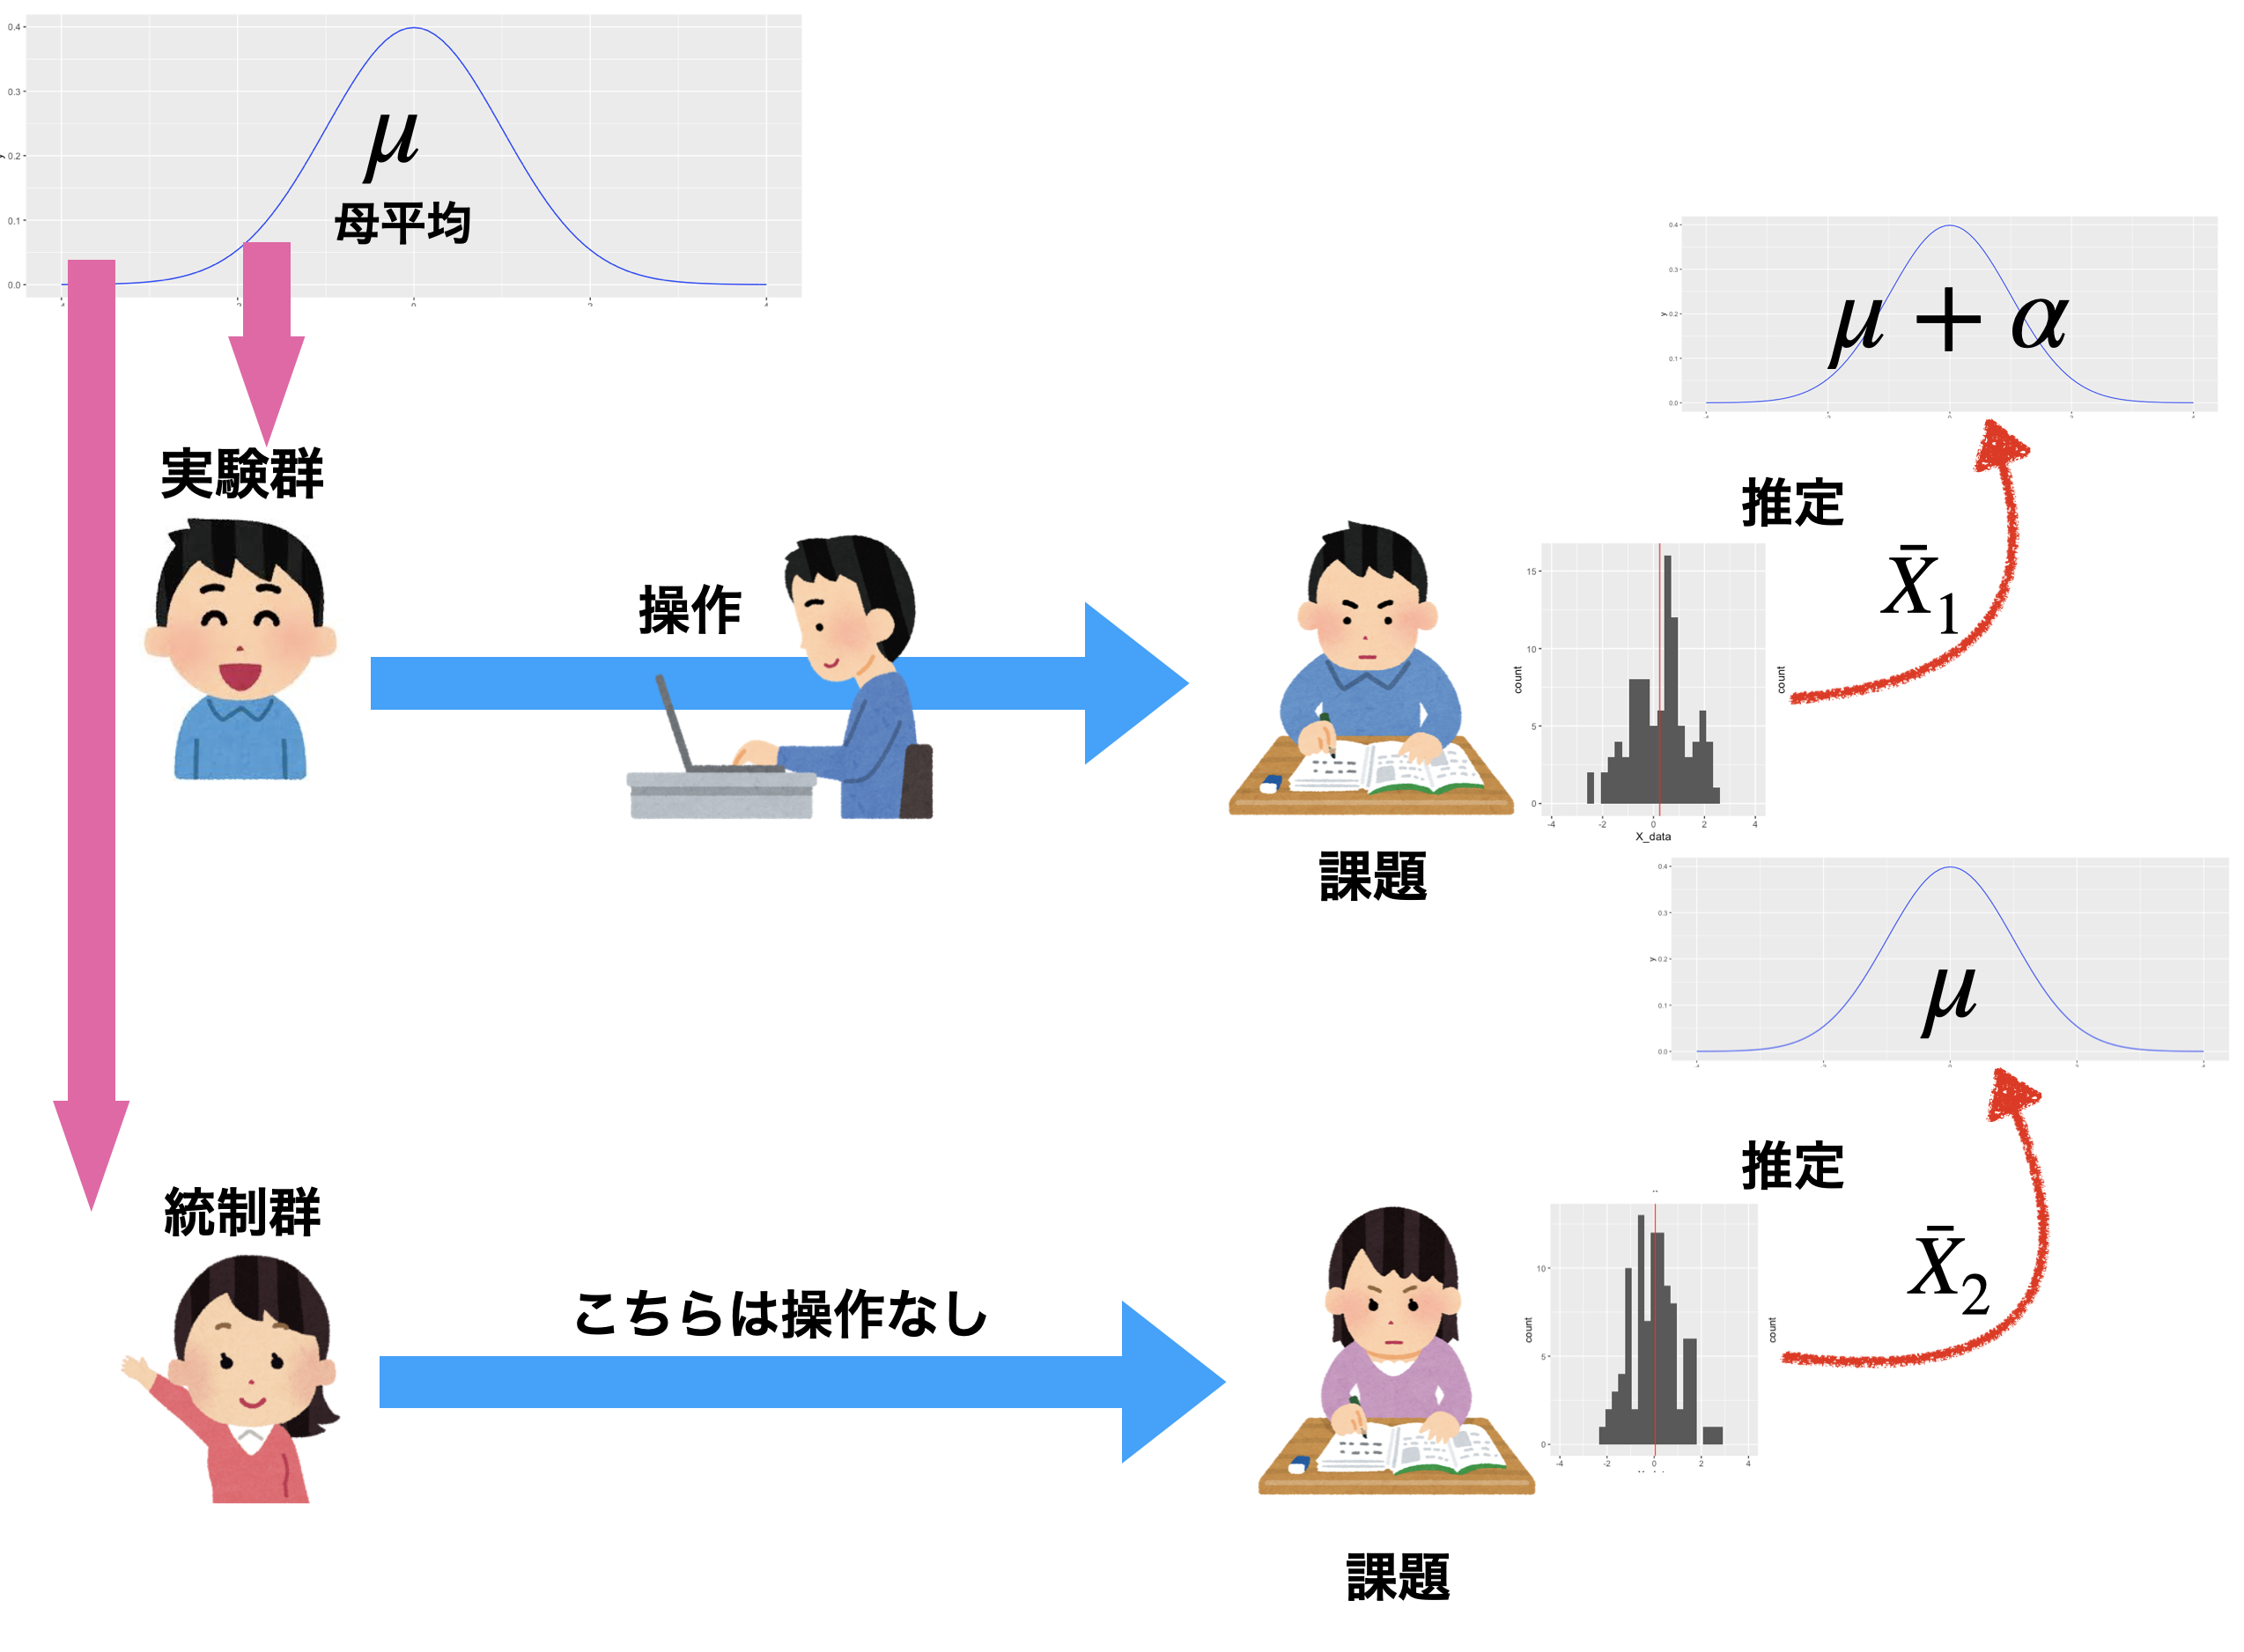
\includegraphics[keepaspectratio,width=0.8\linewidth]{../images/17_estimation_and_test/slide17_4.png}
   \caption{Reprint of Figure \ref{fig::17_05}. One factor Between design with 2 levels.}
   \label{fig::19_02}
\end{figure}


Let's take a look at some specific numerical examples.
% latex table generated in R 4.0.2 by xtable 1.8-4 package
% Wed Sep  2 10:43:49 2020
\input{m20_ttest_escape_06}
Let's assume $n=5$ for this case. Imagine that five participants were randomly assigned to either the experimental or control group. The experimental group completed a cognitive task, followed by a test to measure their memory. The scores from the test are listed in the "value" column. Now, is there a difference in the average scores between the group that completed the cognitive task and the group that did not?

Without modifying the TeX code, please translate the following Japanese text to English:

"Since we do not know the population SD, we use the t-distribution to estimate the population mean from the sample mean. As both the experimental and control groups have n=5, we use the t-distribution with degrees of freedom n-1 = 5-1 = 4 for estimation. Using this, we estimate the population mean of the control group."
From $\bar{X}_{ctl} =20.60$ and $\hat{\sigma_{ctl}}=4.393$,
\[15.145 < \mu_{ctl}<26.055 \]
The Japanese text translates to: "The experimental group has a mean of $\bar{X}_{exp} = 25.20$, without altering the TeX code."
From $\hat{\sigma_{exp}}=6.221$.
\[17.476<\mu_{exp}< 32.924 \]
You are a translator.

Is there any difference? It's subtle! If we estimate the control group to be larger, the sample mean might have been around 26.05, and if we estimate the experimental group to be smaller, the sample mean might have been around 17.48. It's difficult to make a judgment with interval estimation alone.
\subsection{Let's settle it with a hypothesis test}
Let's perform a hypothesis test using the same characteristic as in our previous example: "subtracting one normal distribution from another normal distribution results in another normal distribution". Suppose we draw a random sample from a population that follows the normal distribution $N(\mu,\sigma)$. Then, we know that the sample mean $\bar{X}$ follows the normal distribution $N(\mu,\frac{\sigma}{\sqrt{n}})$. Now, let's consider the difference in sample means between two groups, $\bar{X}_1 - \bar{X}_2$. We know that this difference follows a normal distribution with mean $\mu_1-\mu_2$ and standard deviation $\sigma/\sqrt{\frac{1}{n_1}+\frac{1}{n_2}}$. However, since we do not know the value of $\sigma$, we need to use an unbiased estimator instead. In this case, we have two groups, and using the unbiased variance of either the experimental group or the control group alone would be incorrect. Therefore, we need to combine both groups and use their combined unbiased variance.
\[ \hat{\sigma^2}_{pooled} = \frac{(n_1-1)\hat{\sigma_1^2}+(n_2-1)\hat{\sigma_2^2}}{n_1+n_2 - 2}\]
You are a translator. Tex code will not be modified. Please translate the following Japanese text into English: 

"We will use "pooled", which means combined, for estimation of variance. Since this is an estimation of the standard deviation of the distribution of differences, the positive square root of this will be used as an estimate."
You can use the equation \[\hat{\sigma}_{pooled} = \sqrt{\frac{(n_1-1)\hat{\sigma_1^2}+(n_2-1)\hat{\sigma_2^2}}{n_1+n_2 - 2}}\] to obtain the results.

It's getting a little complicated, but using this, we can calculate the statistics as follows.

\[ t = \frac{\bar{X_1}-\bar{X_2}-(\mu_1-\mu_2)}{\sqrt{\frac{(n_1-1)\hat{\sigma_1^2}+(n_2-1)\hat{\sigma_2^2}}{n_1+n_2 - 2}}\sqrt{\frac{1}{n_1}+\frac{1}{n_2}}}\]

Oh, don't close your heart! The mathematical equations are just there to convey the main idea. You may feel overwhelmed by all the text, but you don't need to remember these formulas. In this educational context, we explain them, but in reality, statistical software can give you the answer easily with built-in functions. What's important is to understand the concept, so in the beginning, even if you don't fully understand the mathematical formulas, it's okay to just think "oh, this is something written there." Instead, let us be amazed by the fact that the $t$ equation only contains sample statistics.

Those who thought, "You're lying, aren't there $\mu_1$ and $\mu_2$?" have a keen eye. Indeed, this is an unknown point (that's why it's written in Greek letters), but we will conduct a test using this. In a test, we set a null hypothesis. The null hypothesis assumes that there is no difference, so we assume that "there is no difference between the means of two groups." In other words, $\mu_1=\mu_2$ or $\mu_1-\mu_2=0". You're doing well! Under the null hypothesis, we can set the denominator $\mu_1-\mu_2=0", so we can ...
\[ t = \frac{\bar{X_1}-\bar{X_2}}{\sqrt{\frac{(n_1-1)\hat{\sigma_1^2}+(n_2-1)\hat{\sigma_2^2}}{n_1+n_2 - 2}}\sqrt{\frac{1}{n_1}+\frac{1}{n_2}}}\]
As a result, it has been determined that it can be completely calculated from the sample statistics. Now, let's proceed with the test.
\paragraph{Setting the Hypothesis} You need a null hypothesis and an alternative hypothesis. As mentioned earlier, the null hypothesis is $\mu_1 = \mu_2$, and the alternative hypothesis is its negation, which is $\mu_1 \neq \mu_2$.
\paragraph{Selecting the Test Statistic} Since we are estimating the mean value, the test statistic to use is the $t$-statistic.
\paragraph{Setting the criteria for judgement based on probability} Let's set the significance level $\alpha$ at 5\% for this round as well, determining the outcome of the match based on this.
\paragraph{Calculating the Test Statistic} This is a bit tricky, but according to the formula and assuming the control group is $X_1$ and the experimental group is $X_2$, we have $\bar{X_1}=20.60, \hat{\sigma}_1=4.393, \bar{X_2}=25.20, \hat{\sigma}_2=6.221$.

\[ t = \frac{20.60-25.20}{\sqrt{(4.393^2+6.221^2)/5}} = -1.3506\]

As a translator, my translation of the Japanese text to English is as follows:

Therefore, this follows a t-distribution with degrees of freedom of $(n_1-1)+(n_2-1)=n_1+n_2-2=10-2=8$, without modifying the TeX code. The probability of obtaining a more extreme t-value is now $p=0.1068".
\subsection{Testing and Directionality}
Please note that there is a point of caution here. The null hypothesis in this case was that the population means of the two groups are not equal. "Not equal" can mean that $\mu_1>\mu_2$ or $\mu_1<\mu_2$. When calculating the observed value of the test statistic in this case, we used $\bar{X_1}-\bar{X_2}$ as the numerator, but we could also have used $\bar{X_2}-\bar{X_1}$. If we had used the latter, the value of $t$ would have been 1.3506.

Let's take a look at the reasoning behind the $t$ value we just saw, while looking at the $t$ distribution. In this case, the realized value of $t$ was -1.3506, but when considering the probability of having an even more extreme value, we calculated it using \texttt{1-qt(1.3506,df=8)}, regardless of the sign. In R, this calculation is equivalent to finding the area under the curve up to 1.3506 by subtracting the result from 100\%, as shown shaded in blue on top of the graph in Figure \ref{fig::19_03}. The explanation may seem a bit convoluted due to the double negative inversion, but it is effectively the same as \texttt{qt(-1.3506,df=8)}.

\begin{figure}[ht]
	\centering
	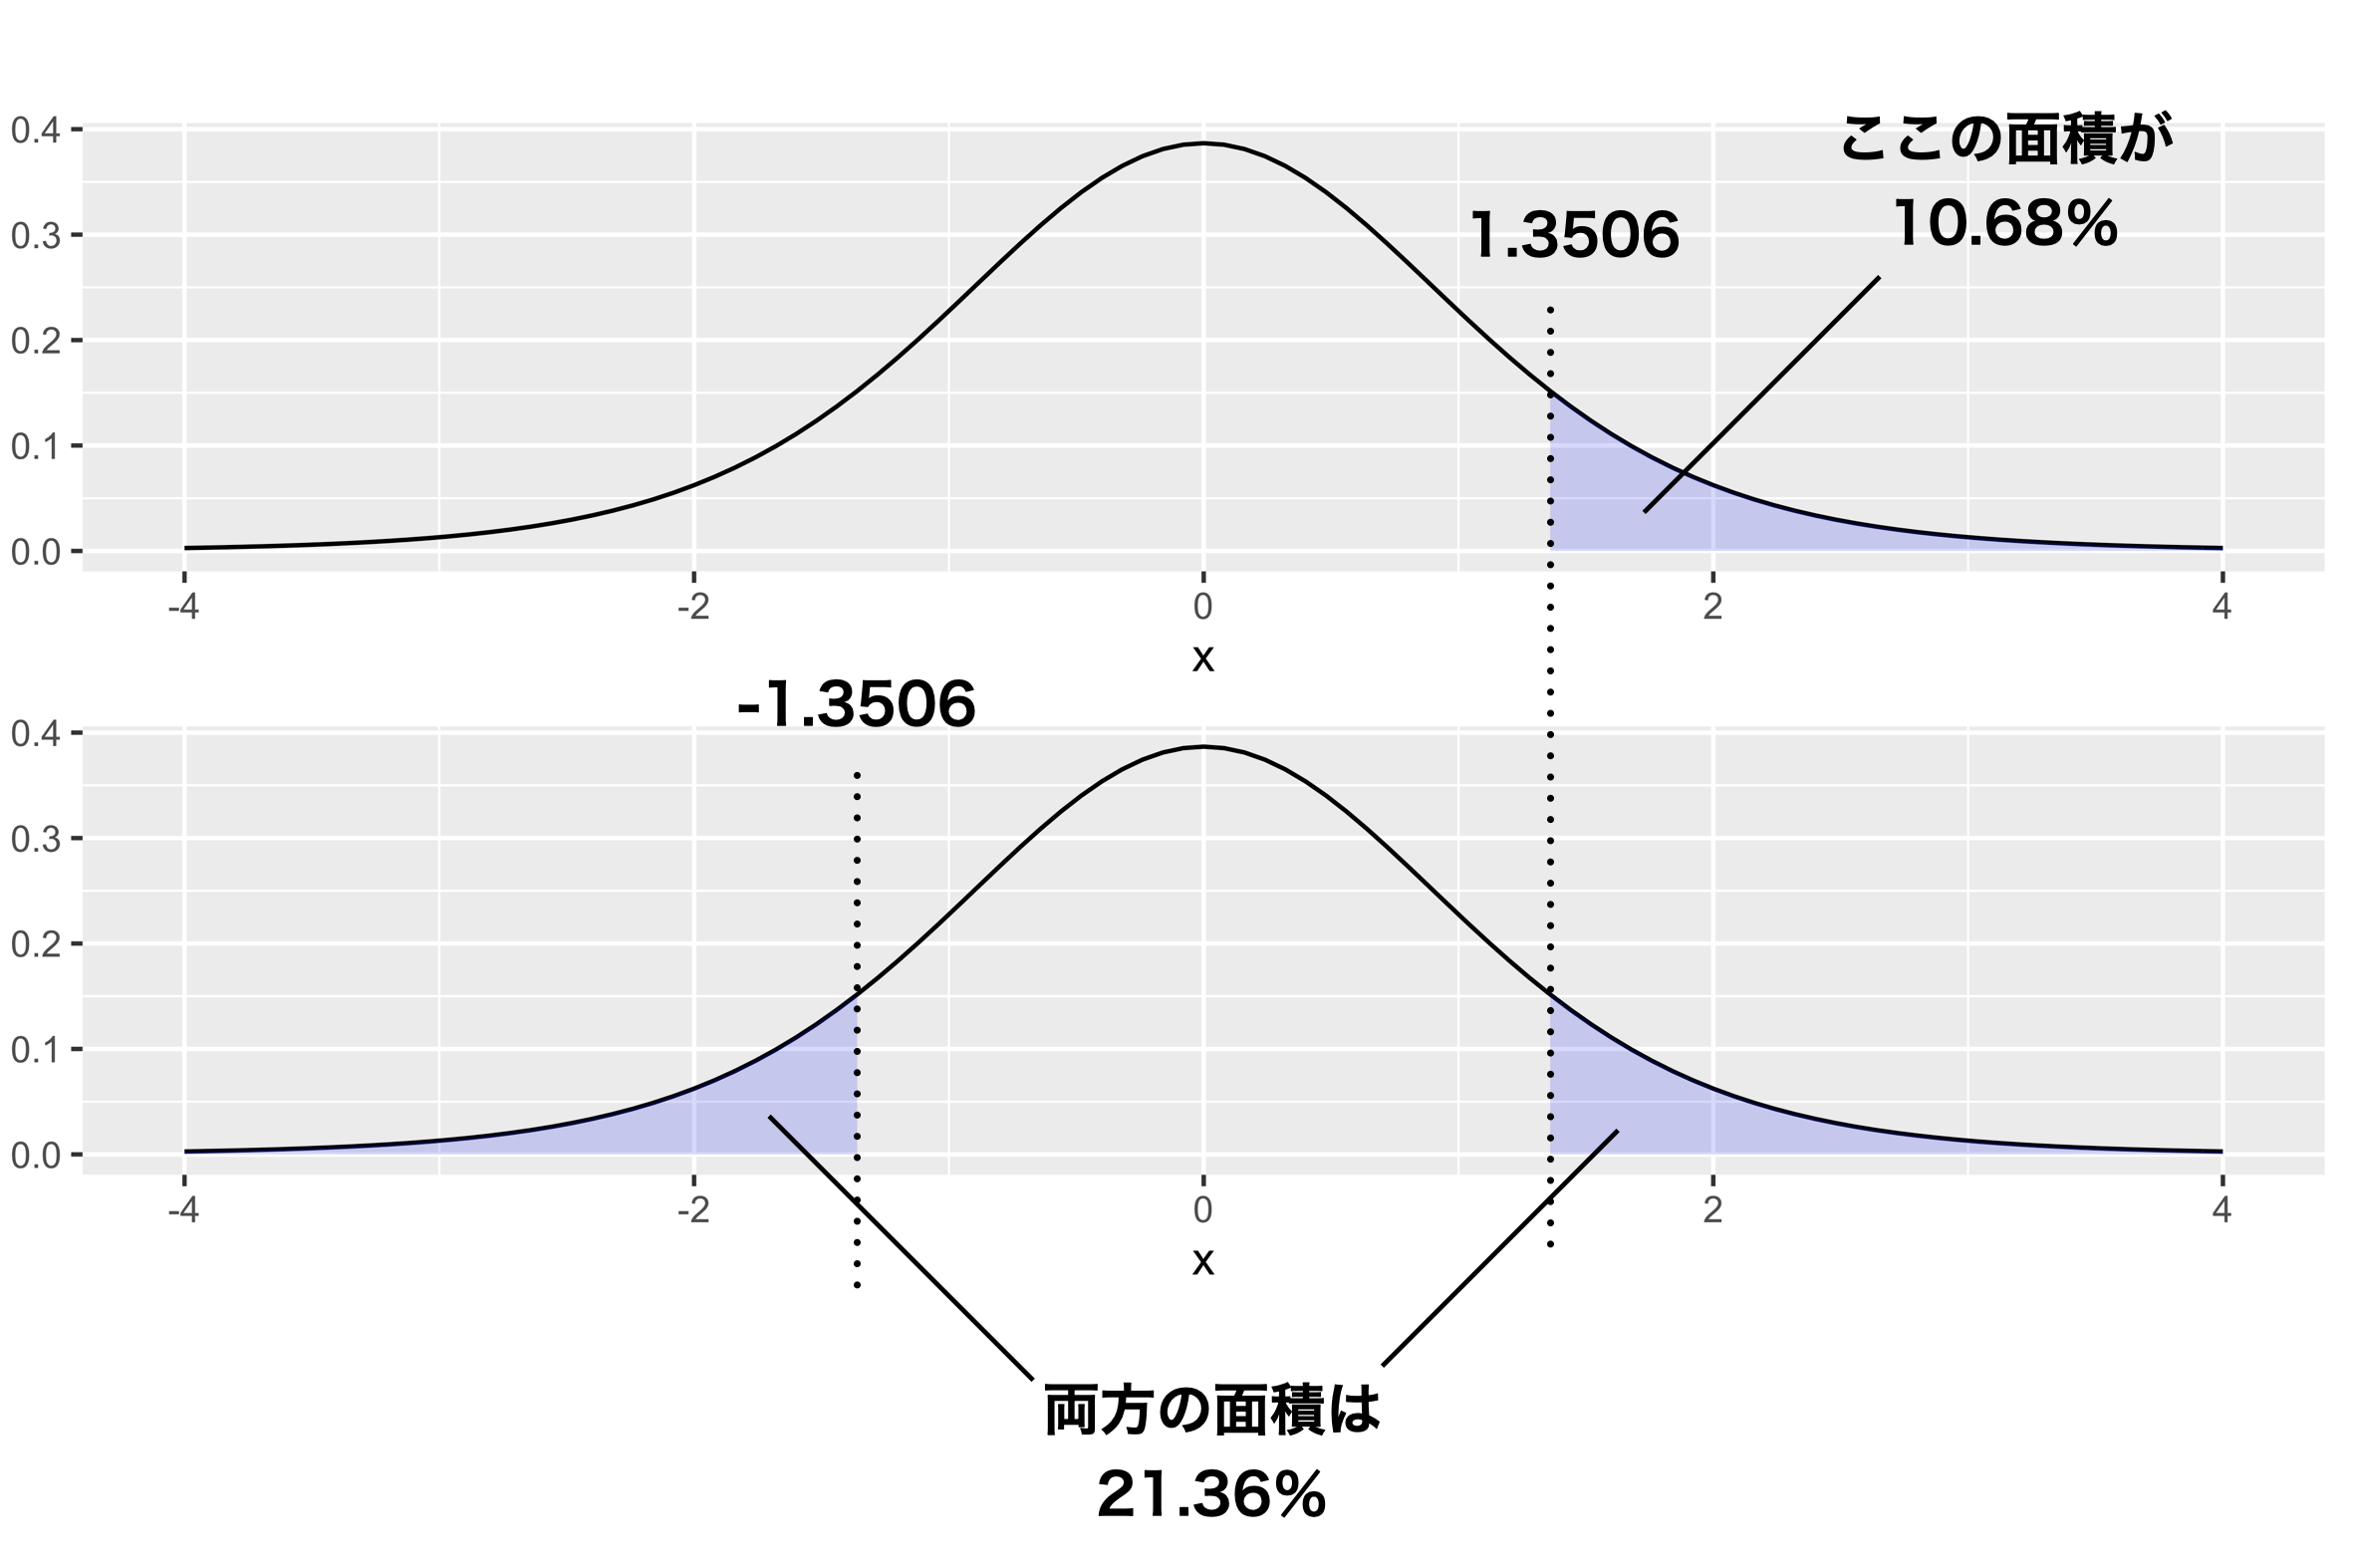
\includegraphics[keepaspectratio,width=0.8\linewidth]{../images/19_NHST2/slide19_02.png}
	\caption{One-tailed test (top) and two-tailed test (bottom)}
	\label{fig::19_03}
\end{figure}


And the value of $t$ is dependent on subtracting the mean of the control group from that of the experimental group, or vice versa, which changes the sign. As the hypothesis did not consider which one to apply, both are possible, meaning there is a possibility of twice the occurrence as indicated in the area under the curve in Figure \ref{fig::19_03} (bottom).

This is called "directionality" in testing, and if it means "one should be larger than the other," then it is sufficient to consider only one side's area. This is called a \keytermE{one-sided test}, and when we conducted the paired t-test in the previous section, we performed a one-sided test assuming a "positive" effect of clinical intervention. However, if there is a possibility that the clinical intervention may worsen the situation, then we would have to double the area under consideration.
\footnote{Even in that case, the conclusion that the 5\% level was significant remains unchanged, since $0.0175\times2=0.035$ is below that level.}

This time, we were only interested in the "difference" between the experimental group and the control group, and we assumed that the experimental manipulation would make a difference, either positive or negative, without knowing which direction it would go. Therefore, we conducted a two-sided test and the probability of encountering $t$ was $p=0.2136$ without altering the TeX code.


Let's summarize. When reporting, it should look like the following.
\begin{quote}
When the difference between the average values of the experimental group and the control group was tested, it was not statistically significant with $t(8)=1.356, p=0.214$.
\end{quote}


For testing the difference between means of two groups, the procedure is as follows. It should be reiterated that the actual calculations are done by a machine, so it is important to have a solid understanding of the procedural knowledge of what the numbers represent and how to interpret the results to make judgments.

Also, since we have seen specific examples of testing here, please try utilizing this technique in your daily life.
If two groups have different means, is it due to chance or not? Can this be generalized? This inferential statistical concept could be applied in many aspects of our daily lives. Once you acquire the knowledge and skills, try to come up with concrete examples and test them. For instance, in a sibling argument such as "Your fries always have the longer pieces, it's not fair!" you could measure the length of both of their fries, calculate the mean, and perform a t-test to determine whether it's just the fries this time or a common occurrence. When the author tested this hypothesis with the fries in a bar, there was no significant difference in the average length of fries among the different tables. Also, they were impressed with how close the length of the fries came to a normal distribution.


\section{Practical application in R; paired t-test}
Let's compute using R specifically.
First, let's test the mean difference of a one-way within-subjects t-test, which is known as a \keytermE{t-test}{tけんてい} for two levels. Although there are tedious calculation formulas, the machine will handle the calculations this time, so be sure to carefully check the output as usual.

As an example, let's use the data of 10 participants in Table \ref{fig::19_01}. Execute the code in \texttt{code:\ref{code:20_08}} to store the original data in an object.
\begin{lstlisting}[language=c++,label={code:20_08},caption={Performing t-test}]
X <- c(34, 25, 13, 21, 13, 26, 19, 12, 19, 19)
Y <- c(35, 30, 16, 27, 20, 28, 16, 14, 18, 21)
t.test(X, Y, paired = T, alternative = "less")
\end{lstlisting}


\paragraph{Code Explanation}
\begin{description}
   \item[1st line] One of the data is assigned to the object \texttt{X} and combined using the function \texttt{c}.
   \item[2nd line] The other data is assigned to the object \texttt{Y}.
   \item[3rd line] Conducting t-test by specifying the data \texttt{X, Y} as arguments and then setting the \texttt{paired} option to \texttt{T}\footnote{\texttt{T} represents TRUE, a special character which indicates true, and its opposite is \texttt{F} which represents FALSE. TRUE and FALSE are logical values that represent two states, true or false, and here represent switches on/off. It means turn on the corresponding switch. It is possible to use capital letters T,F as object names, but since R uses them as reserved words for professional purposes, it is generally advisable to avoid such use.}, and alternative hypothesis as "X is smaller than Y" to conduct a \underline{one-sided test}.
\end{description}

Now, the script was written in an intuitive and easy-to-understand way, but the same thing can also be expressed in a different way (\texttt{code:\ref{code:20_09}}).

\input{m20_ttest_escape_11}
This is the same as before for the first two lines, but...
\begin{description}
   \item[Line 3] Create a data frame from an object. The values of the data are assigned to the variable \texttt{value}, and the variable \texttt{condition} is used to differentiate the values based on conditions. The \texttt{rep} function in \texttt{condition} repeats a specified character or number, and in this case, it creates ten 1s using \texttt{rep(1,10)}. Running only this part of the code will help to understand its operation (see output \ref{RS:out20_02} in R).
      \begin{Rscreen}{Output of rep function}{out20_02}
         \begin{verbatim}
> rep(1,10)
[1] 1 1 1 1 1 1 1 1 1 1\end{verbatim}
      \end{Rscreen}
   \item[Line 4] The variable \texttt{condition} created earlier is converted into a factor type (labeled nominal scale level).
   \item[Line 5] It is a t-test, but with a different format. The tilde \texttt{\~} is used to express the dependent variable as \verb|~| independent variable.  
\end{description}

Here is how to create a data frame, so it would be helpful to see what a data frame looks like (\texttt{R output\ref{RS:out20_03}}).

\begin{Rscreen}{Checking the contents of dat}{out20_03}
	\begin{verbatim}
> dat
   condition value
1        pre    34
2        pre    25
3        pre    13
(omitted)
11      post    35
12      post    30
13      post    16
(omitted)
\end{verbatim}
\end{Rscreen}

The Japanese words that were translated are:

- "datの中身を確認" means "Checking the contents of dat".
- "中略" means "omitted".
- "後略" means "omitted".

During actual data analysis, it is common to either read data files from external sources or analyze data that has already been formatted into data frames. In R, using the tilde to represent the independent and dependent variables is a common way to express functional relationships, so this tutorial explains both ways of using it.

Now, the result obtained is as shown in \texttt{R output \ref{RS:out20_04}}.
\begin{Rscreen}{Output of t.test}{out20_04}
   \begin{verbatim}
Paired t-test
data:  value by condition (value = numerical data, condition = group identifiers)
t = -2.4783, df = 9, p-value = 0.01754
alternative hypothesis: true difference in means is less than 0
95 percent confidence interval:
        -Inf -0.6248331
sample estimates:
mean of the differences (between values in different conditions)
                   -2.4 
\end{verbatim}
\end{Rscreen}


On the third line from the top, there's a value for $t$. Under the null hypothesis, the observed $t$ statistic is $t(9)=-2.4783$, with a corresponding probability of $p=0.01754$. The alternative hypothesis is that the true difference in means is less than 0. Note that R syntax expresses the relationship between the first and the second variable. The one-tailed test is due to specifying \texttt{alternative="less"} in the \texttt{t.test} function. If you use \texttt{alternative="greater"}, the test becomes one-tailed with the opposite direction (prior data score is greater than posterior data score). If you do not specify anything, or set \texttt{alternative="two.sided"}, then a two-tailed test is conducted.

Please refer to the previous chapter (Section $\to$ \ref{m19_NHST2}) to understand how to interpret such results and how to document them in a report.

\section{Practical Application with R: Unpaired t-test}
Next, let's learn how to conduct \keytermE{t-tests} in R, even for cases where no match is available.

We will consider analyzing the data from Table \ref{tbl::19_02} earlier. Without complicated calculations, please input \texttt{code:\ref{code:20_10}} and perform the analysis.
\input{m20_ttest_escape_15}
The contents of the script are similar to earlier. The major difference is that the arguments for the \texttt{t.test} function are not present, and there are no options for \texttt{paired} or \texttt{alternative}. This is because the script is using the default settings, where the R function \texttt{t.test} performs two-sided t-tests for unpaired data by default.

The result should be displayed as shown in \texttt{R output \ref{RS:out20_05}}.
\input{m20_ttest_escape_16}
Please double-check whether the result matches what you calculated by hand last time.

Hmm? The degrees of freedom are 7.195? Wasn't it supposed to be 8 degrees of freedom (experiment group has degrees of freedom of $5-1=4$, and control group has degrees of freedom of $5-1=4$, adding the two gives $4+4=8$)?

\subsection{Welch's Correction}
Yes, the t-test should have 8 degrees of freedom, but it's giving strange numbers. This is because there was another procedure involved in the test that hasn't been explained yet.

Please remember what assumptions were made for the hypothesis test. Setting the null hypothesis as the difference in means being zero is one assumption, but there was an assumption before that. Specifically, it was assumed that the two groups were obtained from a normal distribution and that although there was a difference in the means, the population standard deviation was taken from the same place.

What if this assumption is not true? If we cannot assume a normal distribution in the population, then a t-test cannot be performed. For example, if the data involves differences in annual income or numerical values related to percentages or angles, we cannot assume a normal distribution and therefore cannot perform a t-test. Even if a normal distribution is assumed, if the population standard deviation is different, we may need to reconsider how to estimate it.

This problem is solved by adjusting the degrees of freedom of the $t$ value. The so-called $t$ test used in previous cases was a calculation method that assumed equal variances (which also includes assumptions such as homogeneity of variances), and when this assumption is not met, an adjustment called \textit{Welch's correction} is necessary.

The \texttt{t.test} function in R defaults to returning results with a more lenient assumption, Welch's correction. This means that the function corrects for unequal variances from the start, since checking whether the variances are equal and all that can be cumbersome. The first line of the result even says "Welch Two Sample t-test." With this test, the results are…
\begin{quote}
	A statistically significant difference was not observed between the two groups at $t(7.195)=1.351, p = 0.2178$.
\end{quote}

I will report that\footnote{Since it is a two-sided test, the sign of $t$ does not matter and it is written as negative.}. Let's not only focus on whether there is a difference, but also pay attention to the 95\% confidence interval of the difference. From the results, the 95\% confidence interval of the difference was CI[-12.609577, 3.409577]. Since the difference ranges from -12 to +3 and includes the null hypothesis that the difference is equal to 0, it is not statistically significant.


By the way, if we can assume equal variances, we can use the option of the \texttt{t.test} function as shown in \texttt{code:\ref{code:20_11}}.

\begin{lstlisting}[language=c++,label={code:20_11},caption={Option specification for variance}]
t.test(value ~ condition, data = dat,var.equal = T)
\end{lstlisting}


You can achieve results like the output of \texttt{R} shown in \ref{RS:out20_06}, without modifying the TeX code.

\input{m20_ttest_escape_19}
With this method, even the degrees of freedom are integers (although the test results do not change).

Post-hoc effect size validation
Although the examination has ended, was this experiment "worth the effort"? In other words, we are concerned whether the difference in the population mean is sufficiently large. We do not know the population parameters, but we have been estimating them by using sample statistics for unknown parameters. Therefore, after collecting data, let's consider how much of an effect size this data represents.

You can easily calculate effect size using R without changing the TeX code. While R offers various statistical functions by adding packages, you can also use the \textsf{effsize} package \citep{effsize} to calculate effect size. Please refer to Section \ref{m19_NHST2} for more information on effect size. Here, we introduce a more recommended method for calculating Hedges' g (\texttt{code:\ref{code:20_12}}).

\begin{lstlisting}[language=c++,label={code:20_12},caption={Finding Effect Size}]
# Loading package
library(effsize)
cohen.d(value ~ condition, data = dat, hedges.correction = T)
\end{lstlisting}

First, load the package on the second line (if you don't have this package, you need to download it from the internet and save it locally on your PC), then in the next line, calculate Cohen's d with Hedges' correction.

The result is shown as "R output \ref{RS:out20_07}" in the TeX code without modification.
\input{m20_ttest_escape_21}

As shown by the code \texttt{g estimate: -0.7715342 (medium)}, the estimated value is 0.77 and this is of medium size. It seems that there is a moderate difference, but it may not be significant this time due to the small sample size. If the experiment had been properly designed beforehand, the experimental procedure would have been improved.

Calculation of effect size can also be done retrospectively by considering how much standardized mean difference can be expected from the sample obtained in this study. Of course, it can also be used to design the sample size (how many samples should be taken) by assuming the difference in mean values in advance. In this case, be sure to include the sample effect size obtained here in your report.

\begin{quote}
	A statistically significant difference was not found between the two groups at $t(7.195)=1.351,p = 0.2178$. Additionally, the effect size measured with Hedges' g was 0.77.
\end{quote}


\subsection{Appendix}
I would like to add two additional points in an appendix. If you have the time and interest, please read on.
\paragraph{Calculating the effect size for a paired t-test} When conducting a paired t-test and seeking to calculate the effect size, the paired option should first be turned on as shown in \texttt{code:\ref{code:20_13}}.

There are no Japanese words in this TeX code. It is a code snippet written in English using the LaTeX syntax to display code in a document. The code is in the C++ programming language and is calling the function "cohen.d" with arguments "X" and "Y" and a parameter "paired" set to "TRUE".

You are a translator. However, if you are using tildes in your writing, writing it as \texttt{code:\ref{code:20_14}} will result in a warning in the output, as shown in the following output (\texttt{R output\ref{RS:out20_08}}).
No translation is necessary as this is TeX code for a code block in a LaTeX document. The content appears to be code written in the C++ programming language that includes a function call to a statistics package or library, using the Cohen's d effect size measure for a paired sample design.


\input{m20_ttest_escape_25}
This warning indicates that "the variable for identifying each corresponding individual is not included in the data set, which may result in incorrect results. Please use the following format". To address this, use the format shown in \texttt{code:\ref{code:20_15}}.
\begin{lstlisting}[language=c++,label={code:20_15},caption={cohen.d when there is a correspondence}]
X <- c(34, 25, 13, 21, 13, 26, 19, 12, 19, 19)
Y <- c(35, 30, 16, 27, 20, 28, 16, 14, 18, 21)
dat <- data.frame(condition = c(rep(1, 10), rep(2, 10)), value = c(X, Y))
dat$condition <- factor(dat$condition, labels = c("pre", "post"))
dat$ID <- rep(1:10,2)
cohen.d(value ~ condition | Subject(ID), data = dat, paired = TRUE)
\end{lstlisting}

The point here is to create a variable to identify the ID in the 5th line\footnote{We are duplicating the sequence \texttt{1:10} twice using the \texttt{rep} function. In R, colon-separated numbers represent consecutive numbers.}, and rewrite the formula for calculating effect size in the format suggested by the warning.

How to design examples
In an incompatible t-test, despite an effect size of 0.7, it was not statistically significant. It was suggested that this may be due to a small sample size, but how many data points were needed? By inputting the code in \texttt{code:\ref{code:20_16}} into R, you can get a hint.
\begin{lstlisting}[language=c++,label={code:20_16},caption={power.t.test function}]
power.t.test(power = 0.8, delta = 0.7, sig.level = 0.05)
\end{lstlisting} 

Translation:
- power.t.test: the name of a function
- power: a parameter that sets the desired statistical power for a test
- delta: the minimum effect size that the test is designed to detect
- sig.level: the significance level or the probability of rejecting the null hypothesis when it is true

Here, setting \texttt{delta=0.7} assumes that there is a standardized mean difference of 0.7. This value was used because it was estimated to be around that much based on the results of the post-hoc power analysis conducted earlier. However, estimating a smaller or larger value is also possible. Also, \texttt{power=0.8} was set as the \keytermE{power} which was introduced in Section \ref{TypeI_II_Error} (Pp.\pageref{TypeI_II_Error}). It was aimed to reduce Type II Error, a mistake ($\beta$) of concluding that there is no difference when there actually is, to about 20\% and to have an 80\% chance of making a correct conclusion ($1-\beta=0.8$). The significance level is also 5\% ($\alpha=0.05$, which is set as \texttt{sig.level=0.05} in the script).

Upon viewing the output of this, as shown in \texttt{R output \ref{RS:out20_09}}, we can see the following.
\input{m20_ttest_escape_28}
As mentioned here for an effect size of 0.7 and a power of 0.8, one would want to gather around 33 or 34 participants. Conversely, in this case, only 5 were collected, but using them and setting the code as \texttt{code:\ref{code:20_17}}, the output in \texttt{R} is shown as \ref{RS:out20_10}.

\begin{lstlisting}[language=c++,label={code:20_17},caption={Fixing $n$ with power.t.test}]
power.t.test(n = 5, delta = 0.7, sig.level = 0.05)
\end{lstlisting}


\begin{Rscreen}{Output of power calculation}{out20_10}
	\begin{verbatim}
Two-sample t test power calculation 

n = 5
delta = 0.7
sd = 1
sig.level = 0.05
power = 0.16318
alternative = two.sided

NOTE: n is number in *each* group
\end{verbatim}
\end{Rscreen}

Translation:

-  検定力の出力 (Output of power calculation)
-  二つの標本t検定の検定力計算 (Two-sample t test power calculation)
-  n = 5 (n = 5)
-  delta = 0.7 (delta = 0.7)
-  sd = 1 (sd = 1)
-  sig.level = 0.05 (sig.level = 0.05)
-  power = 0.16318 (power = 0.16318)
-  alternative = two.sided (alternative = two.sided)
-  NOTE: n is number in *each* group (NOTE: n is number in *each* group)

As stated here, the power of the test is 0.16, meaning that even if this study is repeated 100 times, it would correctly detect a significant difference only about 16 times out of those 100 with a sample size of $n=5$. It's like playing a game with bad odds.
\section{Task}
Please submit an Rmd file that includes code for the following calculation. Submissions that cannot be verified to run without bugs solely based on the code provided will not be considered. If you have any questions about how to write the code, please contact the TA for the day or Ms. Kosugi via email to receive guidance.
% \paragraph{課題1 標本統計量と一標本検定}
% 表\ref{exe:20_1}のようなデータが得られたとして，次の各指示に従い，結果について回答してください。
% % latex table generated in R 4.0.2 by xtable 1.8-4 package
% % Fri Oct 16 12:52:58 2020
% \begin{table}[ht]
%     \centering
%     \caption{課題1}
%     \label{exe:20_1}
%     \begin{tabular}{rrrrrrrrrr}
%       \hline
%     56 & 57 & 49 & 45 & 56 & 32 & 56 & 47 & 47 & 41 \\ 
%        \hline
%     \end{tabular}
%     \end{table}
% \begin{enumerate}
%     \item このデータセットの標本分散を計算してください
%     \item このデータセットの不偏標準偏差を計算してください
%     \item このデータセットが正規分布に従う母集団から得られたと考えて，母平均について95\%の区間推定をしてください
%     \item このデータセットが母平均$\mu=50$の正規分布から得られたかどうか，5\%水準で検定してください
% \end{enumerate}

\paragraph{Assignment 1: Paired t-test}
As shown in Table \ref{exe:20_2}, assuming that pre- and post-intervention psychological test results have been obtained, please answer the following instructions regarding the results.
% latex table generated in R 4.0.2 by xtable 1.8-4 package
% Fri Oct 16 12:59:41 2020
\input{m20_ttest_escape_31}

\begin{enumerate}
   \item Please test whether the pre-test score is lower than the post-test score at a significance level of 5%.
\end{enumerate}


Task 2: Unpaired t-test without correspondence.
As indicated in Table \ref{exe:20_3}, assuming that the results of the psychological tests for the control group and the experimental group are available, please answer the following instructions regarding the results.
% latex table generated in R 4.0.2 by xtable 1.8-4 package
% Fri Oct 16 13:05:51 2020
\begin{table}[ht]
	\centering
	\caption{Task 3}
	\label{exe:20_3}
	\begin{tabular}{rrrrrrrrrrr}
		\hline
		Control      & 20 & 21 & 21 & 20 & 21 & 22 & 22 & 22 & 20 & 20 \\
		Experimental & 20 & 18 & 22 & 20 & 21 & 18 & 19 & 21 & 21 & 21 \\
		\hline
	\end{tabular}
\end{table}


\begin{enumerate}
   \item Please perform a t-test assuming equal population variances.
   \item Please perform a t-test without assuming equal population variances.
   \item Regarding this test, please calculate Hedges' g as an effect size.
\end{enumerate}


Task 3: Using the Data from Basic Experiment 1
In the Basic Experiment 1 class, data about social impact was collected.
I believe that there was an investigation into whether or not the "presence or absence of others" affects the "amount of task completion" (although I believe that other variables were also taken into account, here we will focus only on the "amount of task completion").
Please use the data to answer the following questions. Please submit the data used for calculations (or data file) as well.
\begin{enumerate}
   \item Calculate the sample mean value, sample variance, and unbiased variance for both groups with and without others.
   \item Assume that this dataset was obtained from a population that follows a normal distribution and perform a 95% confidence interval estimation for the population mean of each group.
   \item Test the difference between the means of the two groups assuming they were obtained from a population that follows a normal distribution. What are the null and alternative hypotheses?
   \item Conduct the test on the difference between the means of the two groups, report the test statistic, and state the conclusion.
   \item Calculate Hedges' g as an effect size for the test. 
\end{enumerate}



\end{document}
